\apendice{Especificación de Requisitos}

\section{Introducción}

Este anexo contendrá los objetivos de la aplicación y los requisitos que va a tener esta.
Consistirán en breves descripciones de todos los objetivos principales, como se subdividen en objetivos mas cortos para conseguir realizarlos y las funcionalidades implementadas.

Requisitos: Contendrá el que consiste el proyecto y las definiciones de los requisitos y objetivos.

\section{Objetivos generales}
\label{txt:objetivos}

Los objetivos que buscamos con este proyecto son:

\begin{itemize}
\item Construcción del prototipo de procesado de las imágenes:
Con este prototipo la funcionalidad buscada era, hacer las pruebas sobre el código, que mas adelante introduciríamos en la aplicación real, pero así podríamos ajustar los parámetros para que funcionase bien. También de esta forma estaríamos seguros que el proyecto es realizable.

\item Construcción de la aplicación: 
Una vez que tengamos el prototipo funcionando, tendríamos que construir una aplicación para ejecutar de una forma mas profesional que simplemente desde un notebook, esto es algo muy avanzado para un usuario sin experiencia, así facilitar la ejecución sin necesidad de depender del notebook.

\item  Construcción del prototipo para el modo automático:
Como hemos realizado el trabajo en tiempo, hemos optado por acoplar un modo de detección de bordes automatizado, para ver si eramos capaces de detectar los segmentos que detectaría un humano.
El problema de este modo es que algunos segmentos no son casi perceptibles por un humano por lo tanto los que estén mas marcados son los que podremos detectar.

\item Añadir el modo automático a la aplicación: 
Como hemos echo anteriormente con el modo de detección de las lineas pintadas. Esta vez también lo acoplaremos a nuestra aplicación, facilitando la ejecución y aplicación de este modo sobre imágenes que no estuvieran pintadas.
\end{itemize}



\section{Catalogo de requisitos}
El proyecto consiste en:
\begin{itemize}
	\item Construcción del prototipo de procesado de las imágenes.
		\begin{itemize}
			\item Lectura de imagen.
			\item Binarización para detectar las estrías pintadas.
			\item Procesado de la imagen binaria.
			\item Extracción de características.
			\item Procesado de las características.
		\end{itemize}
	\item Construcción de la aplicación.
		\begin{itemize}
			\item Lectura de imágenes y cargar en el panel.
			\item Construcción del panel de pestañas
			\item Construcción del modo de automático para lineas pintadas.
			\item Construcción del modo manual para corregir los errores o editar las lineas que hemos pintado.
			\item Construcción de la pestaña para el modo completamente automático.			
		\end{itemize}
	\item Construcción del prototipo para el modo automático.
		\begin{itemize}
			\item Lectura de la imagen.
			\item Equalizacion de la imagen para distribuir el histograma.
			\item Binarización para extraer bordes.
			\item Procesado de la imagen binaria para limpiar de ruido.
			\item Calculo de las características de la imagen.
			\item Procesado de características.		
		\end{itemize}
\end{itemize}


\section{Especificación de requisitos}
\begin{itemize}
	 
\item RF-1: Construcción de la ayuda en la aplicación.
	\begin{itemize}
		\item RF-1.1: Construcción de los menús donde mostrar las opciones de la ayuda en la aplicación.
		\item RF-1.2: Construcción de la ventana que visualizara el HTML.
	\end{itemize}



\item RF-2: Construcción de las opciones para cargar un proyecto o crear un proyecto.
	\begin{itemize}
		\item RF-2.1: Construcción de los menús donde mostrar las opciones de cargar o crear proyectos en la aplicación. 
		\item RF-2.2: Crear la funcionalidad para escribir un proyecto junto con todos los ficheros necesarios para ello.
		\item RF-2.3: Crear la funcionalidad para leer un proyecto y cargarlo para continuar su edición.
	\end{itemize}

\item RF-3: Guardar un proyecto, este constara de las imágenes original y pintada, estadísticas, CSV con las líneas, fichero de configuración, y tabla \LaTeX .
	\begin{itemize}
		\item RF-3.1: Construcción de los menús donde mostrar las opciones de guardar proyectos en la aplicación. 
		\item RF-3.2: Crear la funcionalidad para guardar un proyecto junto con todos los ficheros necesarios para ello.
	\end{itemize}

\item RF-4: Detectar las estrías de dieta contenidas sobre la imagen.
	\begin{itemize}
		\item RF-4.1: Construcción de los botones que implementaran las opciones de calcular las estrías dependiendo del modo de la aplicación. 
		\item RF-4.2: Crear la funcionalidad para los botones de calcular las estrías en un proyecto junto con pintar sobre la imagen los segmentos detectados.
	\end{itemize}
	
	
\item RF-4.1: Construcción del modo para calcular las estrías pintadas en las imágenes.
	\begin{itemize}
		\item RF-4.1.1: Seleccionar el color de las estrías pintadas que queremos detectar.
		\item RF-4.1.2: Seleccionar la orientación de la imagen, la longitud mínima que debe ignorar y el numero de repeticiones que quiere para calcular los segmentos.
		\item RF-4.1.3: Pedir a la aplicación que use el algoritmo implementado para la detección de las estrías pintadas.			 
		\item RF-4.1.4: Mostrar los segmentos que ha calculado con el algoritmo en el panel donde se muestra la imagen.
	\end{itemize}

\item RF-4.2: Construcción del modo manual para corregir los errores o editar las lineas que hemos pintado.
	\begin{itemize}
		\item RF-4.2.1: Pintar lineas sobre la imagen, pero solo sobre el cuadrado, para añadir nuevos segmentos.
		\item RF-4.2.2: Añadir las lineas que ha calculado el algoritmo de detección de estrías pintadas.
		\item RF-4.2.3: Borrar y limpiar la tabla de los segmentos obtenidos, que se corresponden con las estrías.
		\item RF-4.2.4: Pintar, permitir mover y fijar el cuadrado donde queremos pintar las estrías manualmente.
		\item RF-4.2.5: Guardar los segmentos y obtener las estadísticas y mediciones de todos los segmentos que ha calculado el algoritmo y se muestran en la tabla.			
	\end{itemize}
			 
\item RF-4.3: Construcción del modo completamente automático para detectar las estrías en imágenes sin pintar.
	\begin{itemize}
		\item RF-4.3.1: Seleccionar la orientación de la imagen y la longitud mínima que debe ignorar para calcular los segmentos. 
		\item RF-4.3.2: Mandar calcular al algoritmo las estrías que contiene la imagen.
		\item RF-4.3.3: Mostrar los segmentos que ha calculado con el algoritmo en el panel donde se muestra la imagen.					
		\item RF-4.3.4: Pintar, permitir mover y fijar el cuadrado donde queremos quedarnos con las estrías.
	\end{itemize}
\end{itemize}					

\subsection{Diagrama de casos de uso}
El diagrama que contiene los caso de uso de nuestra aplicación esta contenido en la figura \ref{fig:diagramCasosUso}.	

El diagrama extendido del caso de uso 4 esta contenido en la figura \ref{fig:diagramCasosUso4}.


\begin{figure}[h]
\centering
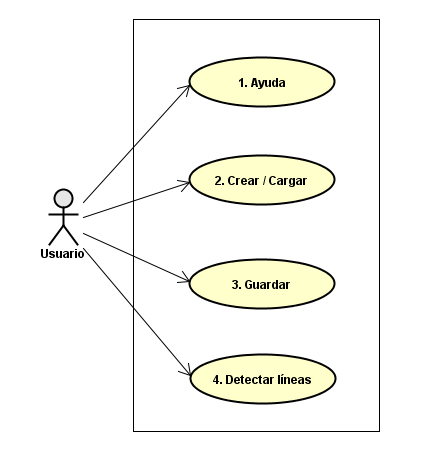
\includegraphics[width=.99\textwidth]{DiagramaCasosUsoGeneral}
\caption{Diagrama general de casos de uso.}
\label{fig:diagramCasosUso}
\end{figure}

\begin{figure}[h]
\centering
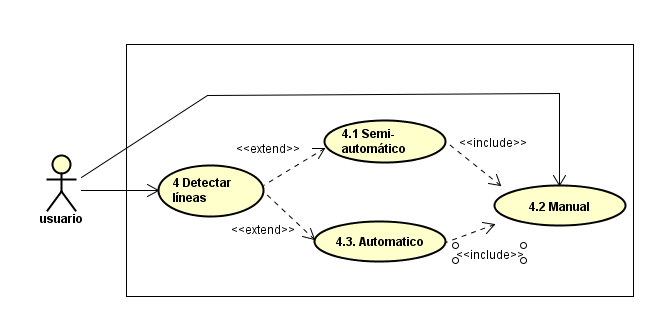
\includegraphics[width=.99\textwidth]{DiagramaCasosUsoCaso4}
\caption{Diagrama de casos de uso extendido.}
\label{fig:diagramCasosUso4}
\end{figure}
 
A partir del diagrama principal y el diagrama extendido, se han diseñado las siguientes tablas de los diagramas de casos de uso, se muestran en las siguientes figuras, \ref{tab:tablacaso1}, \ref{tab:tablacaso2}, \ref{tab:tablacaso3}, \ref{tab:tablacaso4} y este se subdivide en \ref{tab:tablacaso4.1}, \ref{tab:tablacaso4.2} y \ref{tab:tablacaso4.3}.

\begin{table}[]
\centering
\caption{Tabla del caso de uso 1}
\label{tab:tablacaso1}
\begin{tabular}{@{}
>{\columncolor[HTML]{FFFFFF}}p {.25\textwidth} p {.75\textwidth}@{}}
\toprule
\textbf{Caso de uso 1}   & Mostrar ayuda de la aplicacion                                                                                                                                                  \\ \midrule
\textbf{Versión}         & 1                                                                                                                                                                               \\ \midrule
\textbf{Autor}           & Ismael Tobar García                                                                                                                                                             \\ \midrule
\textbf{Requisitos}      & \begin{tabular}[c]{@{}l@{}}RF-1\\ RF-1.1\\ RF-1.2\end{tabular}                                                                                                                  \\ \midrule
\textbf{Descripción}     & \begin{tabular}[c]{@{}l@{}}El usuario podrá consultar la ayuda de la aplicación, para\\ aprender o para consultar algún aspecto que considere\\ oportuno.\end{tabular}            \\ \midrule
\textbf{Precondiciones}  & No tiene                                                                                                                                                                        \\ \midrule
\textbf{Acciones}        & \begin{tabular}[c]{@{}l@{}}1 Ejecutar la aplicación.\\ 2 Abrir el menú principal de la parte superior.\\ 2.1 Seleccionar de la pestaña desplegable la opción ayuda\end{tabular} \\ \midrule
\textbf{Postcondiciones} & Se abrirá una ventana emergente con la ayuda.                                                                                                                                   \\ \midrule
\textbf{Excepciones}     & No pueden saltar                                                                                                                                                                \\ \midrule
\textbf{Importancia}     & Baja                                                                                                                                                                            \\ \bottomrule
\end{tabular}
\end{table}




\begin{table}[]
\centering
\caption{Tabla del caso de uso 2}
\label{tab:tablacaso2}
\begin{tabular}{@{}
>{\columncolor[HTML]{FFFFFF}}p {.25\textwidth} p {.75\textwidth}@{}}
\toprule
\textbf{Caso de uso 2}   & Mostrar ayuda de la aplicacion                                                                                                                                                                                                                                                                                                                                                      \\ \midrule
\textbf{Versión}         & 1                                                                                                                                                                                                                                                                                                                                                                                   \\ \midrule
\textbf{Autor}           & Ismael Tobar García                                                                                                                                                                                                                                                                                                                                                                 \\ \midrule
\textbf{Requisitos}      & \begin{tabular}[c]{@{}l@{}}RF-2\\ RF-2.1\\ RF-2.2\\ RF-2.3\end{tabular}                                                                                                                                                                                                                                                                                                             \\ \midrule
\textbf{Descripción}     & El usuario podrá cargar o abrir un proyecto ya existente para su edición.                                                                                                                                                                                                                                                                                                           \\ \midrule
\textbf{Precondiciones}  & \begin{tabular}[c]{@{}l@{}}Para cargar proyecto: Que exista un proyecto.\\ Para nuevo proyecto: Que exista la imagen a cargar.\end{tabular}                                                                                                                                                                                                                                         \\ \midrule
\textbf{Acciones}        & \begin{tabular}[c]{@{}l@{}}1 Ejecutar la aplicacion.\\ 2 Abrir el menú principal:\\ 2.1 Seleccionar nuevo proyecto.\\ 2.1.1 Buscar la imagen que queremos analizar.\\ 2.1.2 Abrir la imagen seleccionada previamente.\\ 2.2 Seleccionar abrir proyecto:\\ 2.2.1 Buscar el proyecto existente que queremos abrir.\\ 2.2.2 Abrir el directorio previamente seleccionado.\end{tabular} \\ \midrule
\textbf{Postcondiciones} & Se tiene que crear la ventana con la imagen y las opciones disponibles.                                                                                                                                                                                                                                                                                                             \\ \midrule
\textbf{Excepciones}     & \begin{tabular}[c]{@{}l@{}}No exista el proyecto seleccionado \\ No sea una imagen valida\end{tabular}                                                                                                                                                                                                                                                                              \\ \midrule
\textbf{Importancia}     & Alta                                                                                                                                                                                                                                                                                                                                                                                \\ \bottomrule
\end{tabular}
\end{table}


\begin{table}[]
\centering
\caption{Tabla del caso de uso 3}
\label{tab:tablacaso3}
\begin{tabular}{@{}
>{\columncolor[HTML]{FFFFFF}}p {.25\textwidth} p {.75\textwidth}@{}}
\toprule
\textbf{Caso de uso 3}   & Guardar un proyecto desde la aplicación.                                                                                                                                                                                                                                                                                                                                              \\ \midrule
\textbf{Versión}         & 1                                                                                                                                                                                                                                                                                                                                                                                     \\ \midrule
\textbf{Autor}           & Ismael Tobar García                                                                                                                                                                                                                                                                                                                                                                   \\ \midrule
\textbf{Requisitos}      & \begin{tabular}[c]{@{}l@{}}RF-3\\ RF-3.1\\ RF-3.2\end{tabular}                                                                                                                                                                                                                                                                                                                        \\ \midrule
\textbf{Descripción}     & El usuario podrá guardar los datos calculados en un proyecto.                                                                                                                                                                                                                                                                                                                         \\ \midrule
\textbf{Precondiciones}  & \begin{tabular}[c]{@{}l@{}}El usuario deberá haber ejecutado alguno de los tres\\ modos disponibles y tener la tabla con estrías que guardar.\end{tabular}                                                                                                                                                                                                                           \\ \midrule
\textbf{Acciones}        & \begin{tabular}[c]{@{}l@{}}1 Ejecutar la aplicacion.\\ 2 Cargar o abrir proyecto\\ 3 Ejecutar alguno de los tres modos.\\ 3.1 Modo semiautomático para estrías pintadas.\\ 3.2 Modo automático para imágenes sin pintar.\\ 3.3 Modo manual de deteccion de estrías.\\ 4 Hacer click sobre el menú o botón de guardar.\\ 5 Seleccionar un directorio sobre el que guardar\end{tabular} \\ \midrule
\textbf{Postcondiciones} & \begin{tabular}[c]{@{}l@{}}Se tiene que crear un directorio llamado Proyecto que \\ contenga todos los ficheros que componen a este.\end{tabular}                                                                                                                                                                                           \\ \midrule
\textbf{Excepciones}     & \begin{tabular}[c]{@{}l@{}}Si tenemos abierto los ficheros CSV del proyecto nos\\ dirá que no puede guardar\end{tabular}                                                                                                                                                                                                                                                             \\ \midrule
\textbf{Importancia}     & Alta                                                                                                                                                                                                                                                                                                                                                                                  \\ \bottomrule
\end{tabular}
\end{table}


\begin{table}[]
\centering
\caption{Tabla del caso de uso 4}
\label{tab:tablacaso4}
\begin{tabular}{@{}
>{\columncolor[HTML]{FFFFFF}}p {.25\textwidth} p {.75\textwidth}@{}}
\toprule
\textbf{Caso de uso 4}   & Detectar las estrías de dieta contenidas en la imagen.                                                                                                                                                                                                                                                                                                                                                          \\ \midrule
\textbf{Versión}         & 1                                                                                                                                                                                                                                                                                                                                                                                                               \\ \midrule
\textbf{Autor}           & Ismael Tobar García                                                                                                                                                                                                                                                                                                                                                                                             \\ \midrule
\textbf{Requisitos}      & \begin{tabular}[c]{@{}l@{}}RF-4\\ RF-4.1\\ RF-4.2\end{tabular}                                                                                                                                                                                                                                                                                                                                                  \\ \midrule
\textbf{Descripción}     & \begin{tabular}[c]{@{}l@{}}El usuario podrá detectar las estrías que aparezcan en \\ la imagen para producir las estadísticas y todas las\\  salidas generadas con esto.\end{tabular}                                                                                                                                                                                                                           \\ \midrule
\textbf{Precondiciones}  & \begin{tabular}[c]{@{}l@{}}Debe haber una imagen cargada sobre la que calcular\\  las estrías.\end{tabular}                                                                                                                                                                                                                                                                                                     \\ \midrule
\textbf{Acciones}        & \begin{tabular}[c]{@{}l@{}}1 Ejecutar la aplicación.\\ 2 Cargar un proyecto o abrir uno nuevo.\\ 3 Determinar por que modo vamos calcular las estrías.\\ 3.1 Dependiendo del modo debemos seguir unos\\  pasos u otros.\\ 3.2 Procederemos a ejecutar el algoritmo correspondiente.\\ 3.3 Podremos visualizar que estrías han sido detectadas.\\ 3.4 Habilitaremos las funcionalidades de guardar.\end{tabular} \\ \midrule
\textbf{Postcondiciones} & \begin{tabular}[c]{@{}l@{}}Debemos haber detectado la mayoría de las estrías\\ que contienen las imágenes.\end{tabular}                                                                                                                                                                                                                                                                                         \\ \midrule
\textbf{Excepciones}     & \begin{tabular}[c]{@{}l@{}}No puede saltar ninguna ya que lo hemos preparado\\ para esto.\end{tabular}                                                                                                                                                                                                                                                                                                          \\ \midrule
\textbf{Importancia}     & Alta                                                                                                                                                                                                                                                                                                                                                                                                            \\ \bottomrule
\end{tabular}
\end{table}

\begin{table}[]
\centering
\caption{Tabla del caso de uso 4.1}
\label{tab:tablacaso4.1}
\begin{tabular}{@{}
>{\columncolor[HTML]{FFFFFF}}p {.25\textwidth} p {.75\textwidth}@{}}
\toprule
\textbf{Caso de uso 4.1} & \begin{tabular}[c]{@{}l@{}}Ejecución del modo semi-automático para detectar\\ las estrías ya pintadas.\end{tabular}                                                                                                                                                                                                                                                               \\ \midrule
\textbf{Versión}         & 1.0                                                                                                                                                                                                                                                                                                                                                                               \\ \midrule
\textbf{Autor}           & Ismael Tobar García.                                                                                                                                                                                                                                                                                                                                                              \\ \midrule
\textbf{Requisitos}      & \begin{tabular}[c]{@{}l@{}}RF-4.1\\ RF-4.1.1\\ RF-4.1.2\\ RF-4.1.3\\ RF-4.1.4\end{tabular}                                                                                                                                                                                                                                                                                        \\ \midrule
\textbf{Descripción}     & \begin{tabular}[c]{@{}l@{}}El usuario ejecutar el cálculo de estrías pintadas \\ sobre la imagen de forma automática.\end{tabular}                                                                                                                                                                                                                                                \\ \midrule
\textbf{Precondiciones}  & Tener cargada una imagen                                                                                                                                                                                                                                                                                                                                                          \\ \midrule
\textbf{Acciones}        & \begin{tabular}[c]{@{}l@{}}1 El usuario deberá seleccionar el color en el que\\    están pintadas las estrías.\\   2 El usuario deberá seleccionar una longitud mínima\\    que ignorara el algoritmo.\\   3 El usuario deberá seleccionar la orientación de la\\    imagen.\\   4 El usuario deberá seleccionar el número de \\    repeticiones que puede ejecutar.\end{tabular} \\ \midrule
\textbf{Postcondiciones} & Pintar los segmentos detectados en la imagen.                                                                                                                                                                                                                                                                                                                                     \\ \midrule
\textbf{Excepciones}     & \begin{tabular}[c]{@{}l@{}}No puede saltar ninguna ya que los botones se activan\\ solo cuando ha seleccionado todos los pasos bien.\end{tabular}                                                                                                                                                                                                                               \\ \midrule
\textbf{Importancia}     & Alta                                                                                                                                                                                                                                                                                                                                                                              \\ \bottomrule
\end{tabular}
\end{table}

\begin{table}[]
\centering
\caption{Tabla del caso de uso 4.2}
\label{tab:tablacaso4.2}
\begin{tabular}{@{}
>{\columncolor[HTML]{FFFFFF}}p {.25\textwidth} p {.75\textwidth}@{}}
\toprule
\textbf{Caso de uso 4.2} & \begin{tabular}[c]{@{}l@{}} Ejecución del modo manual para pintar estrías en la \\ imagen.\end{tabular}                                                                                                                                                                                                                                                                                                                                                                                                                                                                                                                                            \\ \midrule
\textbf{Versión}         & 1.0                                                                                                                                                                                                                                                                                                                                                           \\ \midrule
\textbf{Autor}           & Ismael Tobar García                                                                                                                                                                                                                                                                                                                                           \\ \midrule
\textbf{Requisitos}      & \begin{tabular}[c]{@{}l@{}}RF-4.2\\   RF-4.2.1\\   RF-4.2.2\\   RF-4.2.3\\   RF-4.2.4\\   RF-4.2.5\end{tabular}                                                                                                                                                                                                                                               \\ \midrule
\textbf{Descripción}     & \begin{tabular}[c]{@{}l@{}}El usuario podrá pintar nuevas estrías sobre la imagen\\ o pintar la imagen desde cero.\end{tabular}                                                                                                                                                                                                                             \\ \midrule
\textbf{Precondiciones}  & Tener una imagen cargada.                                                                                                                                                                                                                                                                                                                                     \\ \midrule
\textbf{Acciones}        & \begin{tabular}[c]{@{}l@{}}1 Deberá seleccionar el botón de corregir líneas\\   1.1 Solo podrá seleccionar puntos dentro del cuadrado.\\   1.1 Deberá seleccionar el inicio de la estría a pintar.\\   1.2 Deberá seleccionar el final de la estría a pintar.\\   2 Deberá hacer click en el botón añadir puntos.\end{tabular} \\ \midrule
\textbf{Postcondiciones} & Ninguna                                                                                                                                                                                                                                                                                                                                                       \\ \midrule
\textbf{Excepciones}     & \begin{tabular}[c]{@{}l@{}}No pueden saltar ya que solo podrá seleccionar puntos\\  dentro de la parte de la imagen contenida en el cuadrado\end{tabular}                                                                                                                                                                                                    \\ \midrule
\textbf{Importancia}     & Media                                                                                                                                                                                                                                                                                                                                                         \\ \bottomrule
\end{tabular}
\end{table}

\begin{table}[]
\centering
\caption{Tabla del caso de uso 4.3}
\label{tab:tablacaso4.3}
\begin{tabular}{@{}
>{\columncolor[HTML]{FFFFFF}}p {.25\textwidth} p {.75\textwidth}@{}}
\toprule
\textbf{Caso de uso 4.3} & Ejecución del modo completamente automático para imágenes sin pintar.                                                                                                                                                                                                                                                                     \\ \midrule
\textbf{Versión}         & 1.0                                                                                                                                                                                                                                                                                                                                       \\ \midrule
\textbf{Autor}           & Ismael Tobar García                                                                                                                                                                                                                                                                                                                       \\ \midrule
\textbf{Requisitos}      & \begin{tabular}[c]{@{}l@{}}RF-4.3\\ RF-4.3.1\\ RF-4.3.2\\ RF-4.3.3\\ RF-4.3.4\end{tabular}                                                                                                                                                                                                                                                \\ \midrule
\textbf{Descripción}     & \begin{tabular}[c]{@{}l@{}}Este modo permitirá al usuario ejecutar el algoritmo\\ para la detección de las estrías en imágenes sin pintar.\end{tabular}                                                                                                                                                                                 \\ \midrule
\textbf{Precondiciones}  & Tener una imagen sin pintar cargada.                                                                                                                                                                                                                                                                                                      \\ \midrule
\textbf{Acciones}        & \begin{tabular}[c]{@{}l@{}}1 El usuario deberá seleccionar una longitud mínima que\\ ignorara el algoritmo.\\   2 El usuario deberá ejecutar el algoritmo que detecta las\\ estrías que hay en la imagen.\\   4 El usuario deberá fijar el cuadrado para quedarse con\\ las estrías detectadas que considere efectivo.\end{tabular} \\ \midrule
\textbf{Postcondiciones} & Pintar los segmentos detectados en la imagen.                                                                                                                                                                                                                                                                                             \\ \midrule
\textbf{Excepciones}     & \begin{tabular}[c]{@{}l@{}}No puede saltar ninguna ya que los botones se activan\\ solo cuando ha seleccionado todos los pasos bien.\end{tabular}                                                                                                                                                                                       \\ \midrule
\textbf{Importancia}     & Alta                                                                                                                                                                                                                                                                                                                                      \\ \bottomrule
\end{tabular}
\end{table}